\documentclass{article}

% if you need to pass options to natbib, use, e.g.:
%     \PassOptionsToPackage{numbers, compress}{natbib}
% before loading neurips_2020

% ready for submission
% \usepackage{neurips_2020}

% to compile a preprint version, e.g., for submission to arXiv, add add the
% [preprint] option:
%     \usepackage[preprint]{neurips_2020}

% to compile a camera-ready version, add the [final] option, e.g.:
%     \usepackage[final]{neurips_2020}

% to avoid loading the natbib package, add option nonatbib:
\usepackage[preprint, nonatbib]{neurips_2020}

\usepackage[utf8]{inputenc} % allow utf-8 input
\usepackage[T1]{fontenc}    % use 8-bit T1 fonts
\usepackage{hyperref}       % hyperlinks
\usepackage{url}            % simple URL typesetting
\usepackage{booktabs}       % professional-quality tables
\usepackage{amsfonts}       % blackboard math symbols
\usepackage{nicefrac}       % compact symbols for 1/2, etc.
\usepackage{microtype}      % microtypography\usepackage{amsmath}
\usepackage{stmaryrd}
\usepackage{multirow}
\usepackage{xcolor}
\usepackage[pdftex]{graphicx}
\usepackage{multirow}
\usepackage{tabularx} 
\usepackage{array}
\usepackage[justification=centering]{caption}
\usepackage{amsmath}

\newcolumntype{P}[1]{>{\centering\arraybackslash}p{#1}}
\newcolumntype{M}[1]{>{\centering\arraybackslash}m{#1}}

\usepackage{stfloats}
% declare the path(s) where your graphic files are
\graphicspath{{figures/}}

\usepackage[sorting=none]{biblatex}
\addbibresource{citations/citations.bib}
\addbibresource{citations/dnn.bib}
\addbibresource{citations/library.bib}

\title{Project Report:\\Fast and Memory-Efficient Coarse-Grained Audio Classification using Deep Neural Network}

\author{
Md Shamim Hussain\\
Department of Computer Science\\
Rensselaer Polytechnic Institute\\
110 8th St.\\ Troy, NY, USA\\
\texttt{hussam4@rpi.edu} \\
\And
Nafis Neehal\\
Department of Computer Science\\
Rensselaer Polytechnic Institute\\
110 8th St.\\ Troy, NY, USA\\
\texttt{neehan@cs.rpi.edu} \\
}

\begin{document}

\maketitle

\begin{abstract}
  Deep neural networks are notorious for their high computational cost and memory requirements. Not only that, often they need specialized hardware for efficient execution. However, for simple tasks such as a coarse-grained classification of sound into superclasses such as speech, music, and noise, one may not be able to spare a lot of computational resources. In this work, we devise a new convolutional network - SwishNetV2 which is fast and memory-efficient, but gets close to big convolutional networks such as VGG16 in terms of classification performance. This architecture improves upon the previous SwishNet architecture and performs well on the CPU with limited memory requirements, similar to its predecessor. We verified the performance of this model on the diverse Audioset dataset, with manually verified gold standard labels. We also devised a method for including data with unchecked noisy labels from AudioSet which improves classification performance. Our annotated dataset is available publicly at \url{https://www.kaggle.com/snirjhar/audioset-speech-music-noise}. The code for our implimentation can be found at \url{https://github.com/shamim-hussain/audioset_coarse_grained_classification}.
\end{abstract}

\section{Introduction}
Music, speech and noise classification and segmentation is an important task because these three types of signals are inherently different in nature \cite{Wolfe2002} and require different types of processing and/or coding schemes. For example, a good compression scheme for speech may not be good for compressing music. Also, the signal processing steps used for these two types of media are likely to be very different. So, correctly identifying the type of media before further processing should be considered a very important task. 

With the advent of widespread use of the internet, it is now possible to build large media databases from user-contributed data. However, labels for the collected data are rarely available. Manual media labeling can be both expensive and time-consuming. So, a reliable method is required to automate the indexing of large media databases. It is intuitive to first classify/ segment the media into broad categories such as speech, music and noise which may be followed by further fine-grained classification/segmentation procedure (for example, into different musical genres). 

The above discussion suggests that it is desirable to bring the classification/segmentation of media into speech, music and noise under a single framework. In recent years deep learning \cite{LeCun2015} algorithms have achieved unprecedented success in numerous classification problems, without any need for careful feature selection. Especially, deep convolutional neural networks have set new frontiers in many fields such as image and audio classification and segmentation. However, deep neural networks are generally known to be more computationally expensive and slower than other more conventional models. These models often need large-scale parallelization in GPUs for faster implementation. Since classification/segmentation is often set as a pre-processing step in an audio processing pipeline, it needs to be fast enough to prevent the delay in further processing. Also, the computational resources are limited in many scenarios such as in mobile devices and embedded systems where it is unreasonable to waste too much resource in the preprocessing step. This is where we put forth our contribution.

Recently, it has been shown that for coarse grained audio classification tasks a fast and lean 1D CNN applied on derived features can show performance close to that of a 2D CNN - the SwishNet architecture \cite{hussain2018swishnet}. Although, this architecture has shown good performance on a clean and less diverse dataset such as the MUSAN \cite{Snyder2015} dataset, it's performance on a more difficult and diversified realistic setting has not been verified. In this work, we further explored the use of lightweight CNN architecutres for audio classification task but in a more diverse and realistic setting - on the AudioSet dataset \cite{gemmeke2017audio}, which is a dataset of 2.1 million annotated audio clips derived from youtube videos. The AudioSet ontology contains 527 different classes, but it does not directly annotate clips into suprerclasses such as speech, music and noise. Instead, it labels each clip with a set of subclasses. We defined these superclasses in the ontology which gives us plausible superclass labels for the clips. However, due to mistakes/missing annotations the actual superclass maybe wrong/ambiguous. So we, manually annotated a set of gold standard labels for around 12000 clips. We devised a new network architecture SwishNetV2 which is an improvement on the SwishNet architecture and directly applies on log mel spectrogram. We verified the performance of this model on the AudioSet dataset with manually verified gold standard labels. We also developed a method for including data with unchecked noisy labels from AudioSet which improves classification performance.

\begin{figure*}[!t]
	\centering
	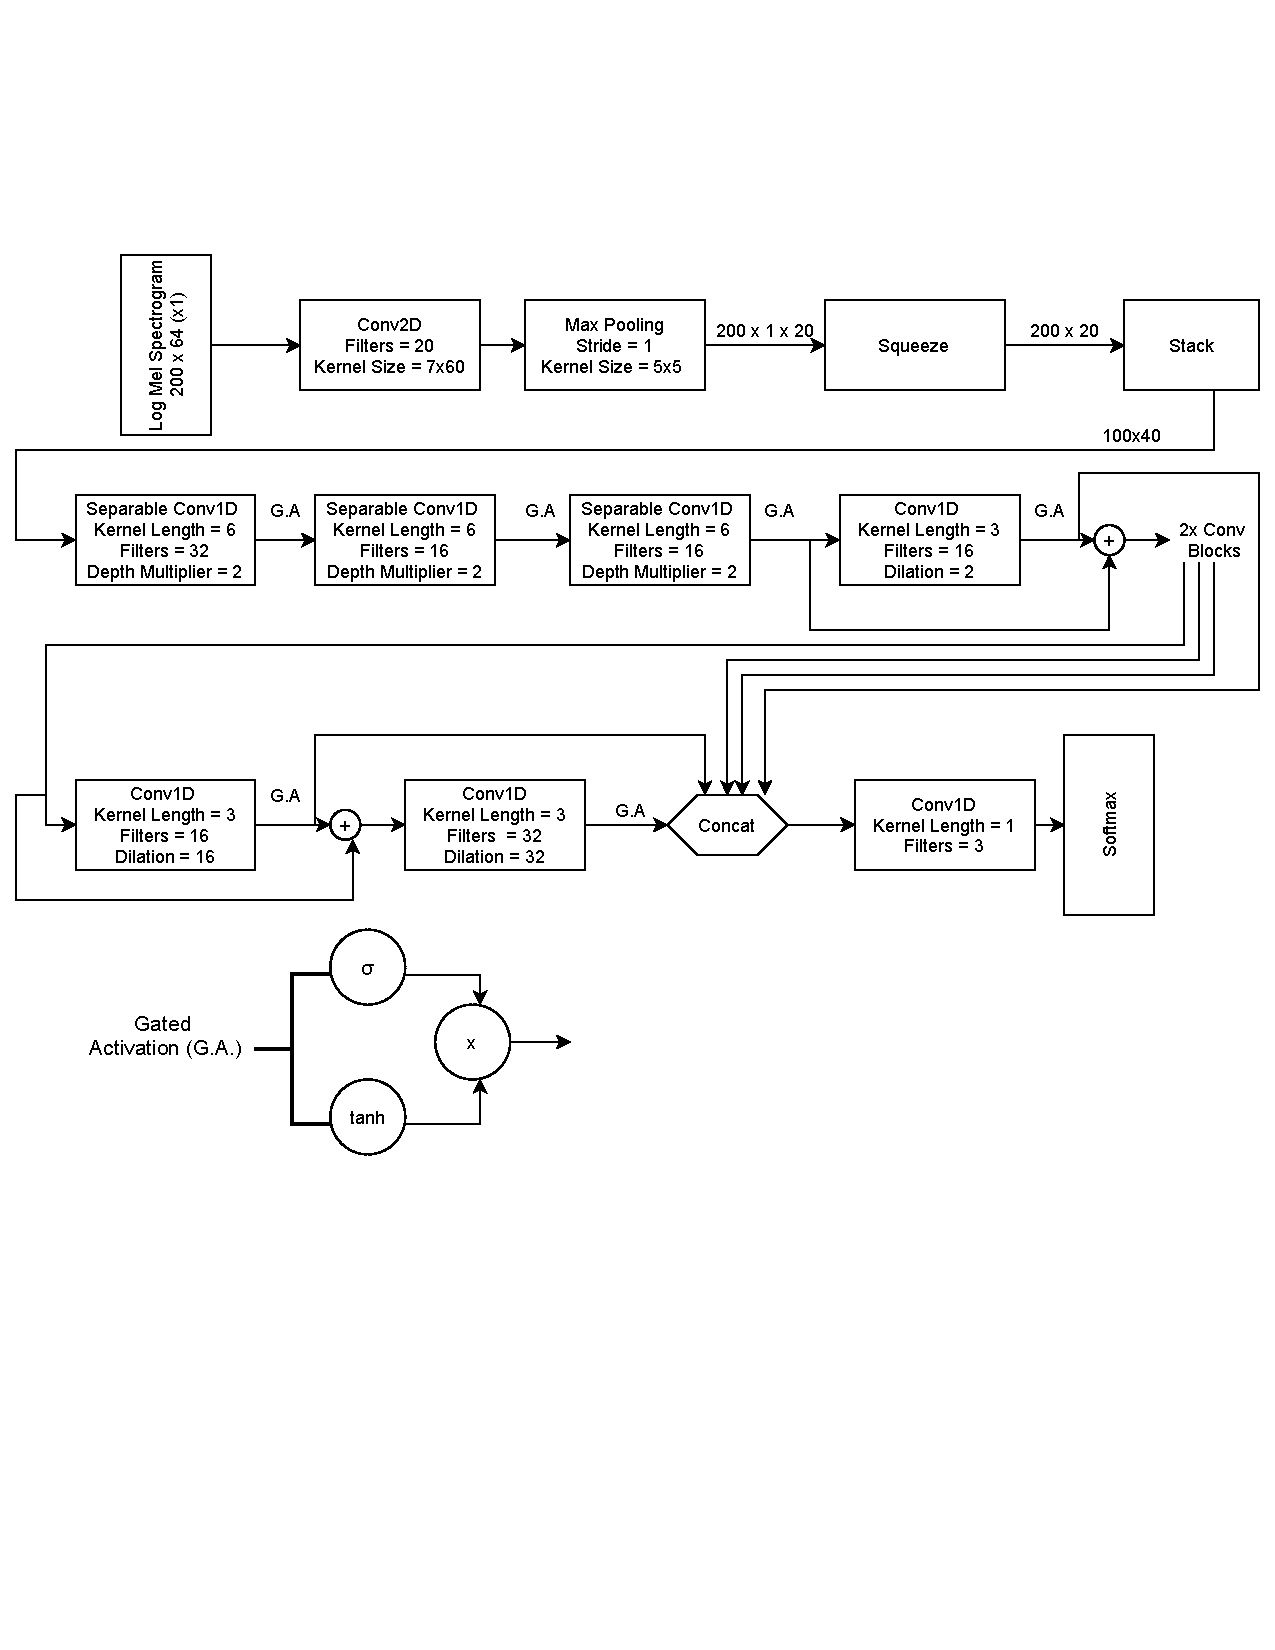
\includegraphics[width=\textwidth, trim= 0 230 0 100, clip]{Network.pdf}
	\caption{Network Architecture of SwishNetV2}
	\label{fig:swishnet}
\end{figure*}

\section{Related Works}
In general, audio content analysis in video parsing can be considered in two directions \cite{srinivasan1999towards, liu1998audio}. One is to discriminate audio streams into different classes such as speech, music, noise etc., the other is to classify audio streams into segments of different speakers. In this paper, our research work in the first direction will be presented. 

There have been many studies on audio content analysis, using different features and different methods \cite{lu2001robust} - Pfeiffer et al \cite{pfeiffer1997automatic}, presented a theoretic framework and application of automatic audio content analysis using some perceptual features. Saunders \cite{saunders1996real}, presented a speech/music classifier based on simple features such as zero crossing rate and short time energy for radio broadcast. When a window size of 2.4s was used, the reported accuracy rate would be 98\%. Scheirer et al \cite{scheirer1997construction} introduced many more features into audio classification and performed experiments with different classification models including GMM (Gaussian Mixture Model), BP-ANN (Back Propagation Artificial Neural Network) and KNN (K-Nearest Neighbor). When using a window of the same size (2.4s), the reported error rate would be 1.4\%. However, it is found that such simple feature-based methods cannot work well when a smaller window is used or more audio classes such as environment sounds are taken into consideration.  

Many other works have been done to enhance audio classification algorithms. In \cite{kimber1997acoustic}, audio recordings are classified into speech, silence, laughter and non-speech sounds, to segment discussion recordings in meetings. The accuracy of the segmentation result using his method varies considerably for different types of recording. In the work by Zhang and Kuo \cite{zhang1999video}, pitch tracking methods are introduced to discriminate audio recordings into more classes, such as songs, speeches over music, with a heuristic-based model. Accuracy of above 90\% is reported. Srinivasan et al [5], try to detect and classify audio that consists of mixed classes, such as combinations of speech and music together with background sound. The accuracy of classification is over 80\%. 

\section{Methodology}
\subsection{Data Collection}
The Audioset \cite{gemmeke2017audio} ontology was used to identify fine-grained sound event classes (source). We combined the fine-grained event classes into 3 major superclasses - speech, music and noise. We define each superclass uniquely by saying that a particular audio segment must not contain events from other superclasses, so that there is no ambiguity in classification. 

We downloaded the annotations of the YouTube video segments. Each segment is assigned multiple sound event tags. We defined plausible superclasses, based on these tags. If a clip contains only the subclasses of a given superclass (speech/music/noise) it is said to belong to that plausible superclass. If the superclass is ambiguous, we ignore that clip. But due to mistakes in annotations, missing annotations and human errors, the actual superclass may still be ambiguous or even wrong. So, the labels assigned at this point are noisy. 

Next, we downloaded YouTube clips in uncompressed wav format which was later compressed by the free lossless audio codec (FLAC). Clips were downloaded from the evaluation set, the balanced training set and the unbalanced training set. We downloaded about 83,600, 10s clips from YouTube.  

To generate ground truth (gold standard) annotations for the clips we manually checked each clip and verified their plausible superclass. If we found that a clip’s superclass was ambiguous/wrong, it was tagged as ``bad'', otherwise it was tagged as ``good''. We performed these manual annotations until we reached 4,000 ``good'' clips for each superclass (speech, music, and noise). Thus, the gold standard (``good'') dataset contains 12,000 annotated unambiguous ground truth labeled clips. Also, the ambiguous (``bad'') labels are also kept for possible future use in automated label clean up. Our annotated dataset, along with unchecked clips is available publicly at \url{https://www.kaggle.com/snirjhar/audioset-speech-music-noise}. 

\subsection{Feature Extraction}
We extracted log mel spectrogram features and energy for each clip. Before that, silence portions of the audio clips were removed, since we do not consider silence in our classification task. Our derived features can be found at \url{https://www.kaggle.com/snirjhar/audioset-derived-features}. The MFCC features used in \cite{hussain2018swishnet} can be easily derived from these features.

\subsection{Network Architecture}
While 1D convolutional networks, like WaveNet \cite{VanDenOord2016b} can operate on raw audio, we trained our network on frame-wise extracted log mel spectrogram because processing raw audio input is infeasible in terms of computational cost and memory requirement for our problem. Note that SwishNet \cite{hussain2018swishnet} operates on MFCC features, which is more specialized but we found that log mel spectrogram features are more informative and thus results in better classification performance.
	
While SwishNet is a 1D convolutional network which operates on frame-wise MFCC features, our model has a single 2D convolutional base followed by 1D convolutions. The rationale behind this is that, the 2D convolution mimics a feature extraction stage, similar to MFCC but at the same time it is trainable. Max Pooling allows for slight invariance in both time and frequency dimensions. Similar to SwishNet, 1D convolutions are carried out along the temporal dimension only. The detailed network architecture of SwishNetV2 is shown in Fig. \ref{fig:swishnet}.
	
	
After the 2D convolutional base we stacked two halves of the signal which effectively halves the time dimension and saves computational time. Similar to the original SwishNet architecture which follows the WaveNet \cite{VanDenOord2016b} architecture, we used multiple layers of causal convolutions to gradually increase the receptive field and gated activation functions \cite{VandenOord2016a} containing sigmoid and tanh functions instead of widely used ReLU activations. The gated activations allow the network to select which information to pass from one time step to the next, just like a gated recurrent network. It also conveniently cuts down the number of feature maps passing from one layer to the next to half.
	
	
At lower layers we used longer filters. Since, longer dense filters are computationally and parametrically costly, here we used separable 1D convolutions \cite{Chollet2016} instead of dense convolution. These longer filters are followed by a series of dialated convolutions which exponentially increases the receptive field of the network.
	
\subsection{A 2D Convolutional Neural Network for Comparison - VGG16}
The most widely used deep learning technique for audio classification is to apply a 2D convolutional network on the spectrogram or other derived features \cite{Sercu2016,Hershey2017,Takahashi2016}. However, to the best of our knowledge, no other deep learning scheme has specifically addressed classification/segmentation into all of the three classes - Music, Speech and noise under a single unified framework. So, for comparison, we sought an established 2D architecture that achieves highest performance for the task at hand.
	
For 2D convolutional networks, we treated the log mel spectrum as a 2D signal and convolutions were done along both frequency and time axes. Among the CNN architectures, we considered, VGG16 \cite{Simonyan2014} performed the best for the task at hand especially its initialized with ImageNet weights. It converges much faster and achieves higher accuracy when initialized with ImageNet weights rather than with random weights. So, this is a case of transfer learning \cite{Oquab2014} from the ImageNet dataset to the AudioSet dataset.
To apply the pre-trained networks on log MFB spectrum, we copied the input along three input channels (Red, Green and Blue) which is equivalent to using a greyscale image. We only kept the convolutional parts of the networks and applied Global Average Pooling to the outputs. Then, we applied two dense layers ending in a softmax output.
\begin{figure*}[!t]
	\centering
	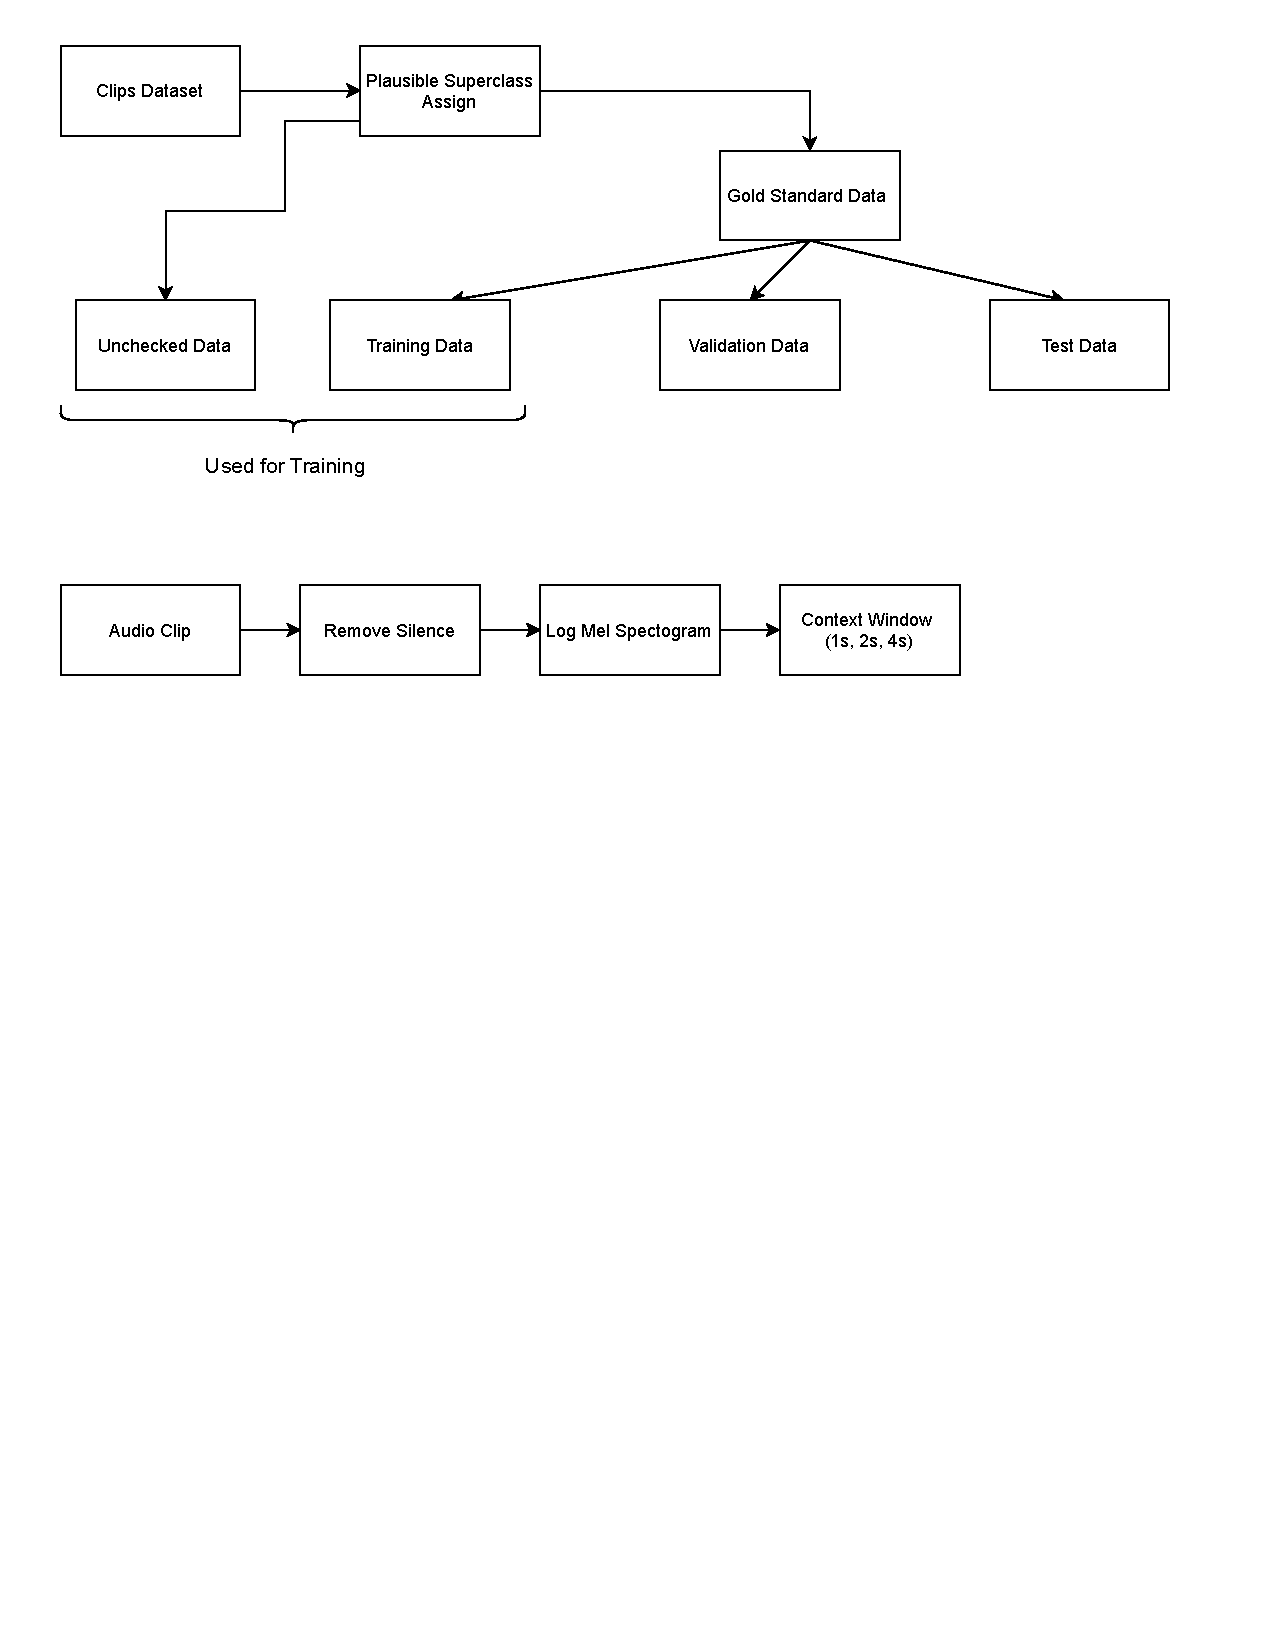
\includegraphics[width=\textwidth, trim= 0 450 0 0, clip]{Pipeline.pdf}
	\caption{Data preparation and feature extraction pipeline}
	\label{fig:pipeline}
\end{figure*}

\section{Results and Discussions}
\subsection{Description of the Dataset}
The AudioSet dataset \cite{gemmeke2017audio} is compiled from annotated youtube videos, which must be collected from original youtube IDs. Often, if the content is not available on youtube, that particular clip must be ignored. It consists of approximately 5.8 thousand hours of audio in 527 categories.

We downloaded around 83.6k audio clips. We encoded all the audio files into 22 kHz FLAC format. Our gold standard dataset contains 12,000 annotated ground truth labeled clips. There were also 66.5k unchecked clips.

\subsection{Evaluation Strategy}
We randomly split the gold standard dataset into a training and a test set in a stratified manner. 35\% of the clips were selected for the test set. Note that, we will use the unchecked clips with noisy labels in the future either for pretraining, or by refining their labels by some means. We randomly split the gold standard training dataset into 5 equally sized, stratified folds. We assigned only 1 of the folds as the validation set, and others were assigned to the "gold standard training" set. Alongside the gold standard training set, the unchecked were also used for training.

The same preprocessing and data preparation steps were followed for all dataset splits. Silent parts of the files were removed using power thresholding. We segmented the files to form either 1s, 2s or 4s clips with 50\% overlap. The clips were framed into 25ms frames with 15ms overlap. 64 log mel filters were applied to each frame. The pipeline is shown in Fig. \ref{fig:pipeline}.

\subsection{Optimization Strategy}
In order to take advantage of the unchecked data while also not being biased by the noisy labels, we used a combination of pretraining on both unchecked and gold standard training data followed by finetuning on gold standard training data only.

We trained SwishNetV2 for 100 epochs with the AdamW optimizer \cite{loshchilov2017decoupled} and a batch size of 256, 128 and 64 for 1s, 2s, 4s clips respectively on the combined training dataset (unchecked + gold standard training). The initial learning rate was set to 0.0005 and it was reduced by a factor of 0.5 if the validation loss didn't improve for 10 epochs. Finally, we finetuned the model on the gold standard training set for 10 epochs with a learning rate of 0.0005.

VGG16 trained really fast when initialized with ImageNet weights and reached convergence within 10 epochs with the SGD optimizer with learning rate of 0.001 and a momentum of 0.5, on the combined training dataset. Then it was finetuned on the gold standard training set for 1 epoch.

\subsection{Results}



% Table generated by Excel2LaTeX from sheet 'Sheet1'

\begin{table}[!t]
	\centering
	\caption{Network Sizes and Prediction Times per Sample}
	\resizebox{\columnwidth}{!}{
		\begin{tabular}{p{4em}P{2.5em}ccccccP{3em}}
			\toprule[1pt]
			\multirow{4}[5]{4em}{\textbf{Network}} & \multicolumn{1}{c}{\multirow{4}[5]{2.2em}{\textbf{No. of Para-meters}}} & \multicolumn{6}{P{17em}}{\textbf{Prediction Time (ms) per Sample}} & \multirow{4}[5]{1cm}{\textbf{Weight file size}} \\
			
			\multicolumn{1}{p{1cm}}{} &       & \multicolumn{6}{P{17em}}{\textbf{for Different Sample Lengths}} & \multicolumn{1}{c}{} \\
			
			\cmidrule{3-8}    \multicolumn{1}{p{1cm}}{} &       & \multicolumn{2}{P{5em}}{\textbf{0.5s}} & \multicolumn{2}{P{5em}}{\textbf{1.0s}} & \multicolumn{2}{P{5em}}{\textbf{2.0s}} & \multicolumn{1}{c}{} \\
			
			\cmidrule(r{.25em}l){3-4} \cmidrule(r{.25em}l){5-6} \cmidrule(r{.25em}l){7-8}  \multicolumn{1}{p{1cm}}{} &       & \multicolumn{1}{p{1em}}{\textbf{CPU}} & \multicolumn{1}{p{1em}}{\textbf{GPU}} & \multicolumn{1}{p{1em}}{\textbf{CPU}} & \multicolumn{1}{p{1em}}{\textbf{GPU}} & \multicolumn{1}{p{1em}}{\textbf{CPU}} & \multicolumn{1}{p{1em}}{\textbf{GPU}} & \multicolumn{1}{c}{} \\
			
			\midrule[1pt]
			\textbf{GMM} & 92,416 & 1.8   & - & 3.6   & - & 7.2   & - & 370KB \\
			
			\midrule
			\textbf{SNN} & 179,203 & 0.71  & 0.72  & 0.92  & 0.72  & 1.52  & 0.82  & 717KB \\
			
			\midrule
			\textbf{SwishNet-slim} & 5,483 & 0.77  & 1.42  & 0.88  & 1.43  & 1.12  & 1.45  & 22KB \\
			
			\midrule
			\textbf{SwishNet-wide} & 18,267 & 0.9   & 1.45  & 1.1   & 1.45  & 1.65  & 1.45  & 66KB \\
			
			\midrule
			\textbf{MobileNet} & 217,235 & 4.1   & 3.51  & 5.27  & 3.52  & 8.57  & 3.55  & 870KB \\
			\bottomrule
		\end{tabular}
	}%
	\label{tab:speed}%
\end{table}%
\begin{table}[t]
	\centering
	\caption{Overall and Speech/Non-Speech (SNS) Classification Accuracy for Clips of Different Lengths}
	\resizebox{\columnwidth}{!}{
		\begin{tabular}{p{3em}p{4.1em}P{2.2em}P{2.2em}P{2.2em}P{2.2em}P{2.2em}P{2.2em}}
			\toprule
			\multicolumn{2}{p{8em}}{\textbf{Clip Length}} & \multicolumn{2}{M{6em}}{\textbf{0.5s}} & \multicolumn{2}{M{6em}}{\textbf{1.0s}} & \multicolumn{2}{M{6em}}{\textbf{2.0s}} \\
			
			\cmidrule(r{.25em}){1-2} \cmidrule(r{.25em}l){3-4} \cmidrule(r{.25em}l){5-6} \cmidrule(r{.25em}l){7-8} 
			\textbf{Network} &  & \textbf{Overall} & \textbf{SNS} & \textbf{Overall} & \multicolumn{1}{p{1.1em}}{\textbf{SNS}} & \textbf{Overall} & \textbf{SNS} \\
			
			\midrule[1pt]
			\textbf{GMM} &  & 96.53\% & 98.58\% & 97.33\% & 99.05\% & 97.79\% & 99.33\% \\
			
			\midrule
			\textbf{SNN} &  & 97.07\% & 98.87\% & 97.41\% & 99.13\% & 97.71\% & 99.36\% \\
			
			\midrule
			\multirow{2}{4em}{\textbf{Swish-Net-slim}} & \textbf{Undistilled} & 97.64\% & 99.24\% & 98.20\% & 99.60\% & 98.41\% & 99.76\% \\
			
			\cmidrule(l{0.5em}){2-8}          & \textbf{Distilled} & 97.52\% & 99.19\% & 98.22\% & 99.51\% & 98.57\% & 99.70\% \\
			
			\midrule
			\multirow{2}{4em}{\textbf{Swish-Net-wide}} & \textbf{Undistilled} & 97.97\% & 99.37\% & 98.32\% & 99.67\% & 98.65\% & 99.75\% \\
			
			\cmidrule(l{0.5em}){2-8}          & \textbf{Distilled} & 98.05\% & 99.45\% & 98.54\% & 99.71\% & 98.92\% & 99.84\% \\
			
			\midrule
			\multirow{2}{4em}{\textbf{Mobile-Net}} & \textbf{Random} & 98.13\% & 99.43\% & 98.53\% & 99.71\% & 98.95\% & 99.88\% \\
			
			\cmidrule(l{0.5em}){2-8}          & \textbf{Pretrained} & 98.94\% & 99.73\% & 99.24\% & 99.89\% & 99.38\% & 99.96\% \\
			\bottomrule
		\end{tabular}
	}%
	\label{tab:classperm}%
\end{table}%




\begin{table}
	\centering
	\caption{Normalized Confusion Matrices for Clips of Different Lengths (Rows: True Labels, Columns: Predicted labels, Ordering: Speech, Music, and Noise. GST = Trained on Gold Standard Training Set, GST + UT = Trained on Gold Standard and Unchecked Training Set, GST + UT + FT = Trained on Gold Standard and Unchecked Training Set, Fine Tuned on Gold Standard Training Set)}
	%\resizebox{\columnwidth}{!}{
	\begin{tabular}{M{13em}P{6.5em}P{6.5em}P{6.5em}} 
		
		\toprule
		\textbf{Network} & \textbf{1.0s} & \textbf{2.0s} & \textbf{4.0s} \\
		
		
		\midrule
		\textbf{SwishNet(GST)} 
		& $\begin{bmatrix}
		.90 & .05 & .05\\
		.02 & .92 & .06\\
		.02 & .11 & .86
		\end{bmatrix} $
		& $\begin{bmatrix}
		.93 & .03 & .03\\
		.01 & .94 & .05\\
		.02 & .11 & .87
		\end{bmatrix}$
		& $\begin{bmatrix}
		.93 & .03 & .03\\
		.01 & .94 & .05\\
		.03 & .11 & .86
		\end{bmatrix}$ \\
		
		\midrule
		\textbf{SwishNet(GST + UT)}
		& $\begin{bmatrix}
		.97 & .01 & .02\\
		.03 & .91 & .06\\
		.06 & .05 & .89
		\end{bmatrix}$ 
		& $\begin{bmatrix}
		.98 & .01 & .01\\
		.01 & .95 & .04\\
		.06 & .06 & 0.88
		\end{bmatrix}$
		& $\begin{bmatrix}
		.96 & .03 & .01\\
		.00 & .97 & .03\\
		.06 & .08 & .86
		\end{bmatrix}$\\
		
		\midrule
		\textbf{SwishNet(GST + UT + FT)} 
		& $\begin{bmatrix}
		.91 & .03 & .05\\
		.01 & .92 & .07\\
		.01 & .05 & .93
		\end{bmatrix}$ & 
		$\begin{bmatrix}
		.96 & .01 & .03\\
		.01 & .95 & .03\\
		.02 & .06 & .92
		\end{bmatrix}$ 
		& $\begin{bmatrix}
		.95 & .01 & .04\\
		.01 & .95 & .04\\
		.01 & .05 & .94
		\end{bmatrix}$ \\
		
		\midrule 
		\textbf{VGG16 (GST + UT + FT)} 
		& $\begin{bmatrix}
		.94 & .01 & .05\\
		.01 & .94 & .05\\
		.01 & .03 & .95
		\end{bmatrix}$ 
		& $\begin{bmatrix}
		.97 & .01 & .02\\
		.00 & .98 & .02\\
		.02 & .05 & .93
		\end{bmatrix}$ 
		& $\begin{bmatrix}
		.98 & .00 & .02\\
		.00 & .97 & .03\\
		.01 & .03 & .96
		\end{bmatrix}$ \\
		\bottomrule
	\end{tabular}
	%}
	\label{tab:conmat}%
\end{table}

the network structures fixed for all tests. Table \ref{tab:speed} compares the sizes prediction speeds of the three networks as well as the baseline models. To simulate comparison of real-time computational cost, we fixed batch size to 1 for all models and compared their speed on CPU and GPU. Our CPU was Core i7 8700K, a 6 core processor and our GPU was NVIDIA GTX 1080ti and the networks were implemented in PyTorch \cite{paszke2019pytorch}.

We see that, similar to SwishNet, SwishNetV2 is fast on both CPU and GPU. SwishNet is approximately 10 times faster than VGG16 on CPU, due to its low parallelization requirement. Also in terms of number of pamameters and weight file size it is about 1000 times smaller than VGG16.

The classification results are presented in Table \ref{tab:classperm} and \ref{tab:conmat}. We see that SwishNet performs very close to VGG16 in terms of accuracy, with the gap being only around 2\%. The performance improves with increasing clip length. Also we see that the two stage of our training method by training on combined dataset and finetuning on gold standard dataset improves classification performance.

From the confusion matrices, we can see that recall for noise is low for both models, especially for smaller clip lengths, even though the speech/non-non-speech discrimination accuracy is high for all clip lengths. This result indicates that for smaller contextual windows, it is hard to differentiate noise from music. This is because, some of the noises, such as bells tolling or phones ringing are slightly musical in nature and short segments of music may sound like noise. So, a longer context is necessary for discriminating noise from music.

\section{Conclusion and Future Work}
We manually added Gold Standard labels to AudioSet clips for speech, music and noise. We designed an improved version of SwishNet architecture – SwishNetV2 which is applied on log mel spectrum directly and achieved better accuracy. Also, we developed a scheme for training on noisy labels and fine tuning on gold standard dataset and showed that it improves accuracy. We showed that lean, fast CNN such as SwishNetV2 come very close in terms of accuracy to big 2D CNNs such as VGG16, even in such a diverse dataset as AudioSet.

In a future work we intend to include more unchecked data which should result in better performance. Also we intend to utilize unchecked data in a more sophisticated manner. One possibility is distillation from ensemble of models. We intend to add clips from other datasets into training. Possible candidates are FSD50K \cite{fonseca2020fsd50k} and MUSAN \cite{Snyder2015}. Additionally, we intend to try and combine different features, including MFCC, log Mel spectrogram, and also NMF based features.



\printbibliography
\end{document}
